\documentclass[10pt,twocolumn,letterpaper]{article}

\usepackage{cvpr}
\usepackage{times}
\usepackage{epsfig}
\usepackage{graphicx}
\usepackage{amsmath}
\usepackage{amssymb}
\usepackage{subfig}
\usepackage{float}

% Include other packages here, before hyperref.

% If you comment hyperref and then uncomment it, you should delete
% egpaper.aux before re-running latex.  (Or just hit 'q' on the first latex
% run, let it finish, and you should be clear).
\usepackage[breaklinks=true,bookmarks=false]{hyperref}

\cvprfinalcopy % *** Uncomment this line for the final submission

\def\cvprPaperID{****} % *** Enter the CVPR Paper ID here
\def\httilde{\mbox{\tt\raisebox{-.5ex}{\symbol{126}}}}

% Pages are numbered in submission mode, and unnumbered in camera-ready
%\ifcvprfinal\pagestyle{empty}\fi
\setcounter{page}{1}

\begin{document}

%%%%%%%%% TITLE
\title{Museum paintings retrieval and people detection}

\author{Marco Cagrandi\\
University of Modena and Reggio Emilia\\
Department of Engineering Enzo Ferrari\\
{\tt\small 203232@studenti.unimore.it}
% For a paper whose authors are all at the same institution,
% omit the following lines up until the closing ``}''.
% Additional authors and addresses can be added with ``\and'',
% just like the second author.
% To save space, use either the email address or home page, not both
\and
Alessio Ruggi\\
University of Modena and Reggio Emilia\\
Department of Engineering Enzo Ferrari\\
{\tt\small 203689@studenti.unimore.it}
\and
Daniele Lombardo\\
University of Modena and Reggio Emilia\\
Department of Engineering Enzo Ferrari\\
{\tt\small 202214@studenti.unimore.it}
}


\maketitle
%\thispagestyle{empty}

%%%%%%%%% ABSTRACT
\begin{abstract}
   Image processing, retrieval and people detection
   are important computer vision applications.
   Here we present our work on the ``Galleria Estense" dataset which contains
   videos and images from the ``Galleria Estense" of Modena.
   We propose a method to detect and retrieve the paintings, the statues and the people in the 
   museum based on different approaches: one with pure image processing and one 
   with YOLOv3 network, trained with a custom annotated dataset of paintings and statues 
   images. 
\end{abstract}

%%%%%%%%% BODY TEXT
\section{Introduction}

We have tackled the problem of detect paintings, statues and people in a museum (the Galleria Estense).
Our objectives were: rectify the paintings correcting the perspective distortions, retrieve the correct paintings in the dataset, provide a precise segmentation of both detected paintings and statues, sum up all the information we had and link the paintings and the people to a precise room in the museum.
 In order to achieve our results, as further discussed in section 3, many techniques are involved: Image processing topics as edge detection, connected components analysis, relevant ROI detection, object segmentation; image retrieval; deep learning and neural networks. 

\subsection{The dataset}

The dataset contains videos and images from the ``Galleria Estense" of Modena.

We have 208 short videos taken using different cameras, aspect ratios and resolutions. 
Some video was taken with a GoPro camera which introduced some distortion and
some video has frames particularly blurred due to the motion applied to the camera.

We have a database of 95 images that should represents all paintings of the ``Galleria Estense", 
but during the development of the project we realized that many paintings were missing 
and so we had to expand the paintings db adding some paintings taken from the \href{https://www.gallerie-estensi.beniculturali.it/opere/#c-dipinti#c-sculture#l-galleria-estense}{``Galleria Estense" website} to improve the retrival and rectification tasks. We added 25 paintings that are named 
with a fixed suffix ``A" followed by a zero-based sequential identifier, \eg ``A000.jpeg".

Finally the dataset contains also a CSV file with informations for every painting present
in the db, including the position of the painting in the museum as a room number, and also an image
representing the plant of the museum to do the people detection task. When we expanded the 
painting db we expanded the CSV file accordingly to maintain consistency.

\section{Related works}

To detect the paintings and statues in the museum we trained a YOLOv3 network with
our custom annotated dataset. YOLO (acronym for ``You Only Look Once") is an object detection
network able to detect objects in images parsing the image only once, saving computation time w.r.t. 
other detection networks, however maintaining a good degree of precision.
We choosed YOLOv3 because it can achieve good performaces
both in terms of detection and speed as described in YOLOv3 paper \textit{Joseph Redmon and Ali Farhadi} \cite{yolov3}.

After the detection with YOLOv3, we used GrabCut algorithm for segmentation \cite{grabcut}.
GrabCut is an algorithm used for foreground extraction with minimal user interaction.
User should inputs the rectangle which border the object of interest: everything outside this rectangle is considered sure background, while everything inside the rectangle may be both foreground or background.
This minimal user interaction required by GrabCut is reduced to zero in our case, because, in the case of statues, YOLOv3 network inputs the rectangle, while in the case of painting the input ROIs are the one detected in the Painting Detection.


\section{Approach}

The proposed approach involve several elements: Painting detection, Painting retrieval, 
Painting rectification, People detection and Statue detection.

\subsection{Painting Detection}

The first thing to do in order to detect relevant objects is to perform edge detection, but right before we have 
precessed the image with a gaussian filter in order to remove the gaussian noise and a bilateral filter. 
A good method to detect relevant edges is the Canny algorithm \cite{canny}. It has been proposed with the following empirically determined thresholds 

\begin{table}[h!]
\begin{center}
\begin{tabular}{|l|c|}
\hline
\multicolumn{2}{|c|}{Thresholds}  \\
\hline
Low & High \\
\hline
400 & 400 \\ 
\hline
\end{tabular}
\caption{Canny thresholds}
\end{center}
\end{table}

with a Sobel operator \cite{otsu} with aperture of 5. With low threshold and high threshold set to an equal value, we don't accept weak edges, even if connected with strong edges.

The next step is to perform a Dilation 3x3 followed by an Erosion (Closing), in order to 
connect the edges of the same relevant object, and to detect the connected components in the output image 
thus obtaining a list of ROIs.
In order to discard unrelevant ROIs, we have set some rules that have to be satisfied in order to be considered
a relevant ROI: 
\begin{gather*}
	ratio_{ROI} =  \frac{max(width_{ROI}, height_{ROI})}{min(width_{ROI}, height_{ROI})} <  3 \quad (1)\\
	area_{ROI} > 0.015 \cdot area_{frame} \quad (2)\\ 
	max\_overlap = 0.8 \quad (3)
\end{gather*}

If the overlap is greater than the threshold, the bigger ROI survives.

We then propose an optional optimization, named \textbf{otsu\_optimization} and activated with the 
{\tt otsu\_opt\_enabled} flag set to True,
\begin{gather*}
	otsu\_th(ROI) > 1.3 \cdot otsu\_th(frame) \quad (4)
\end{gather*}
 where \(otsu\_th(x)\) is the function that computes the Otsu threshold. 
This optimization helps when it comes to discard the ROIs containing \eg wall sections,
but sometimes affects the paintings that are overexposed to the light.

\begin{figure}
    \centering
    \subfloat[Original frame]{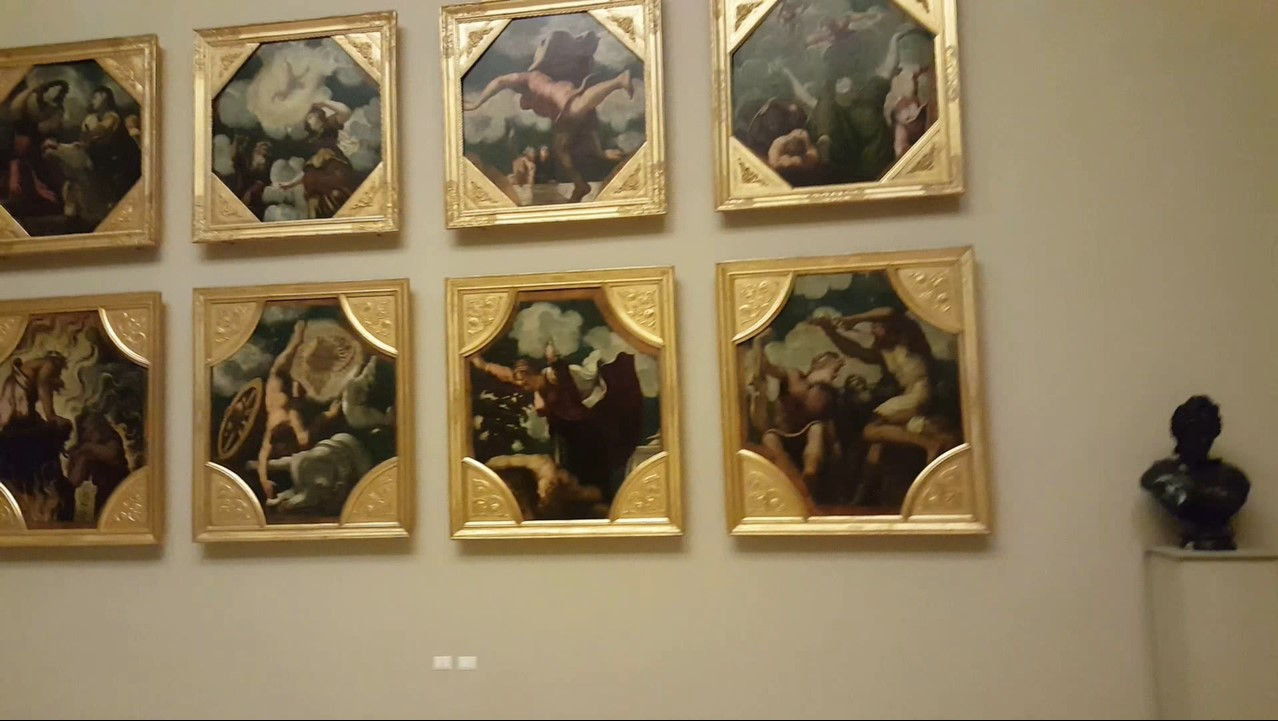
\includegraphics[width=0.6\linewidth]{frame.jpg}}\\
    \subfloat[Canny edge detection]{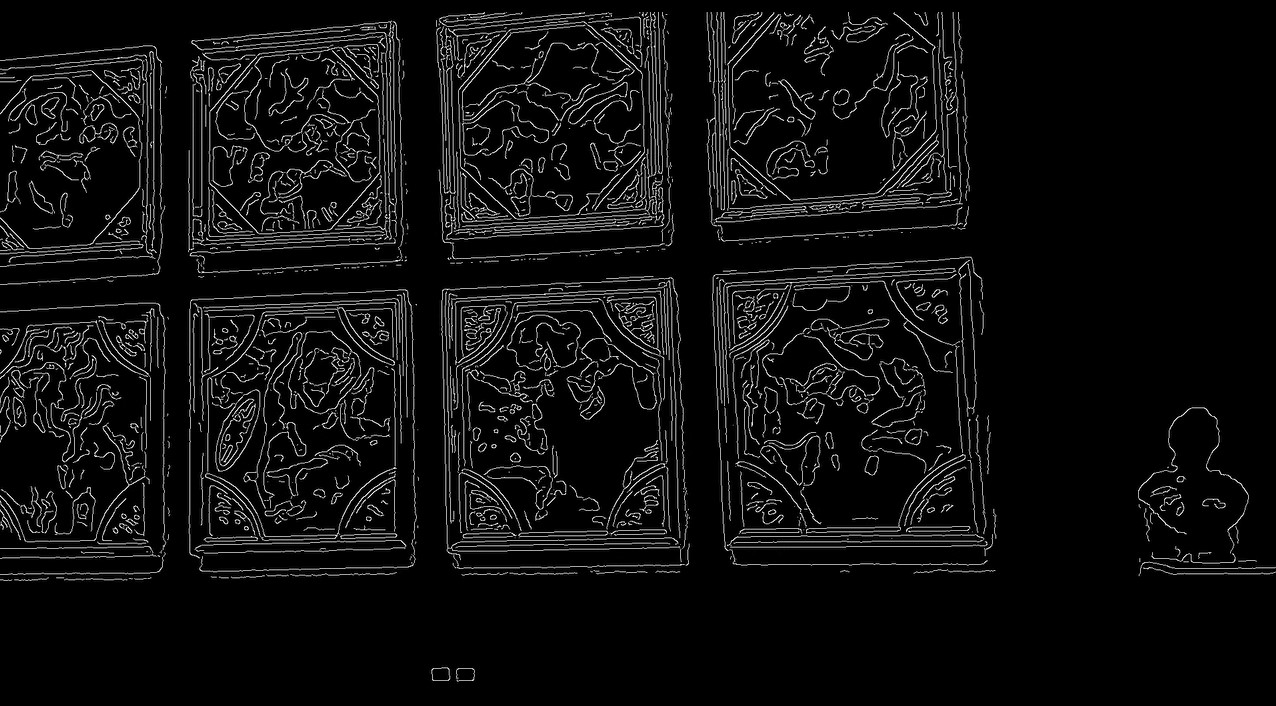
\includegraphics[width=0.6\linewidth]{canny_out.jpg}}\\
    \subfloat[Closing results]{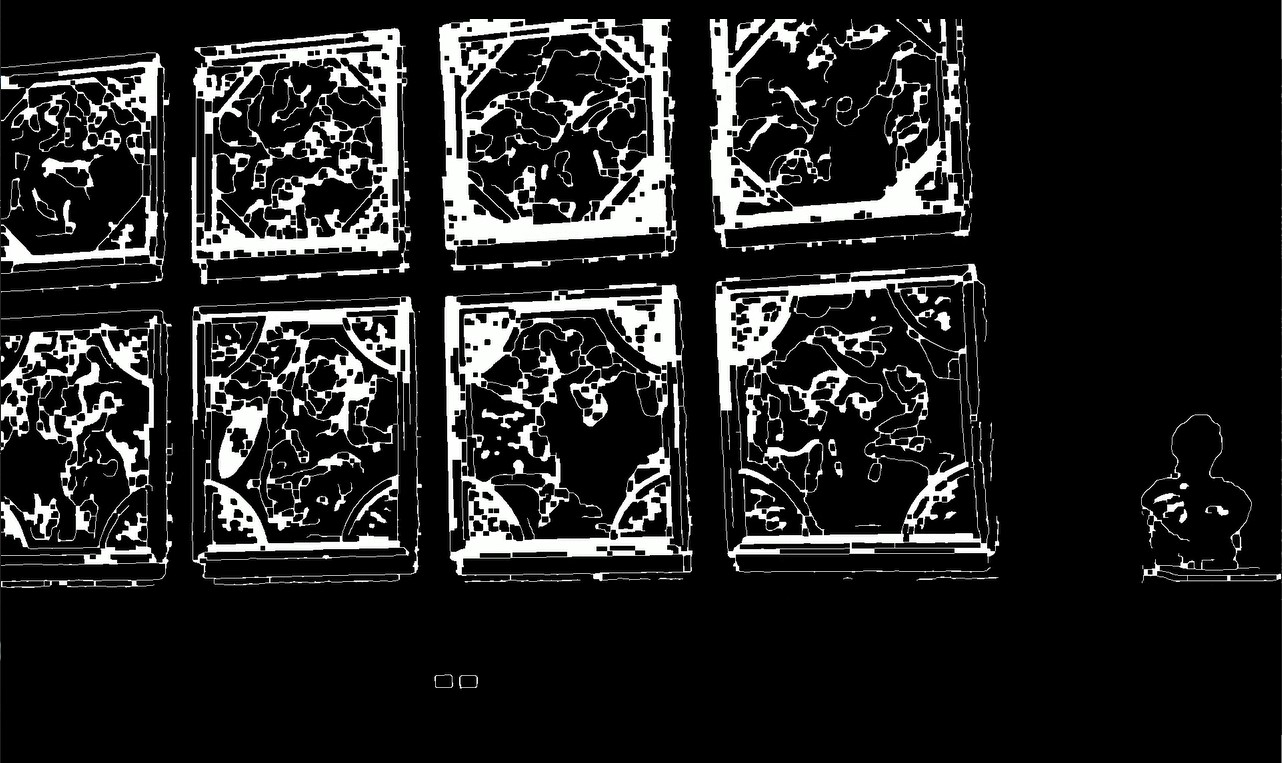
\includegraphics[width=0.6\linewidth]{closing_canny.jpg}}\\
    \subfloat[Detected connected components]{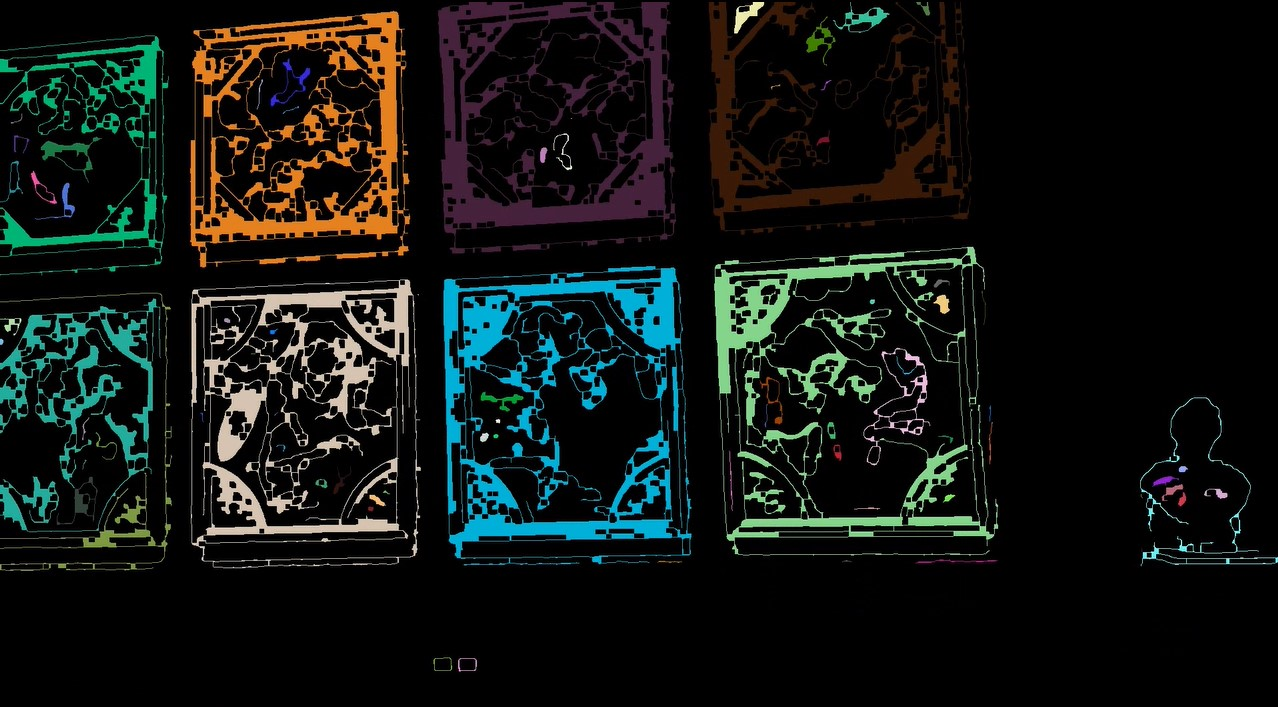
\includegraphics[width=0.6\linewidth]{connected_components.jpg}}\\
    \subfloat[Connected components ROIs]{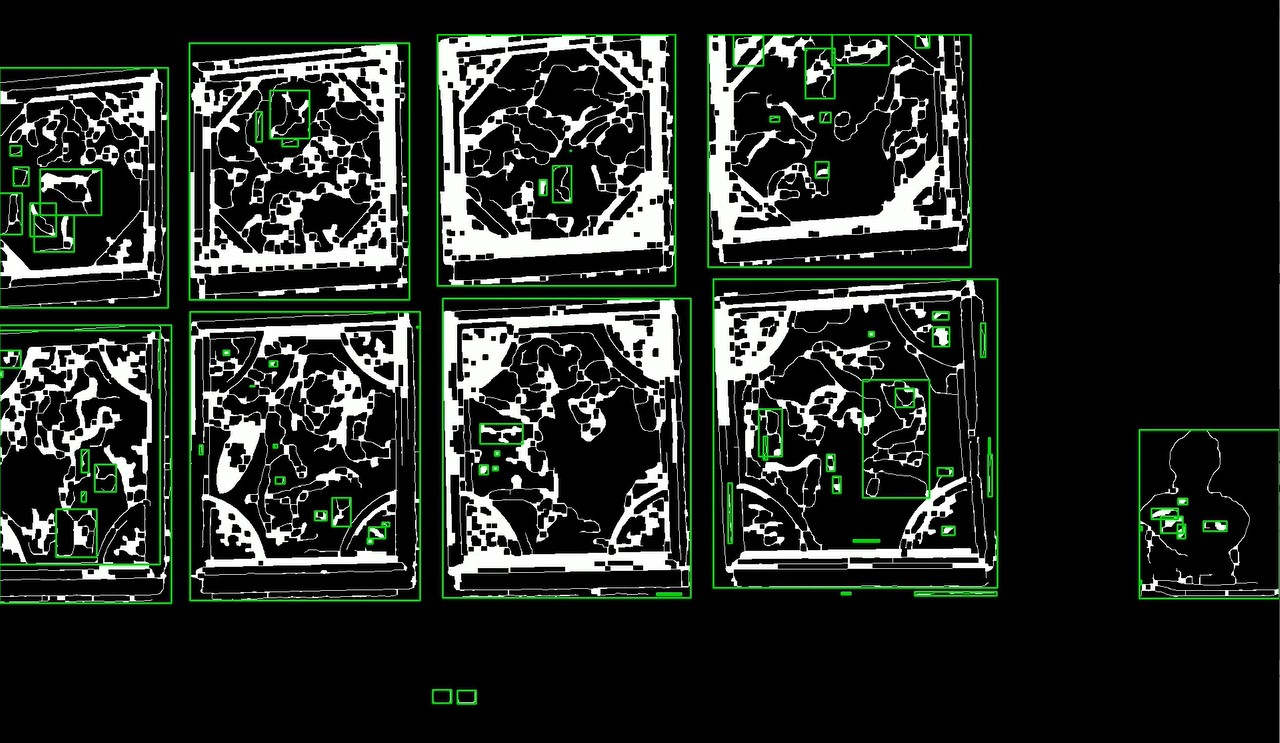
\includegraphics[width=0.6\linewidth]{components_rois.jpg}}\\
    \subfloat[Relevant ROIs; in green the discarded ROIs due to the overlap]{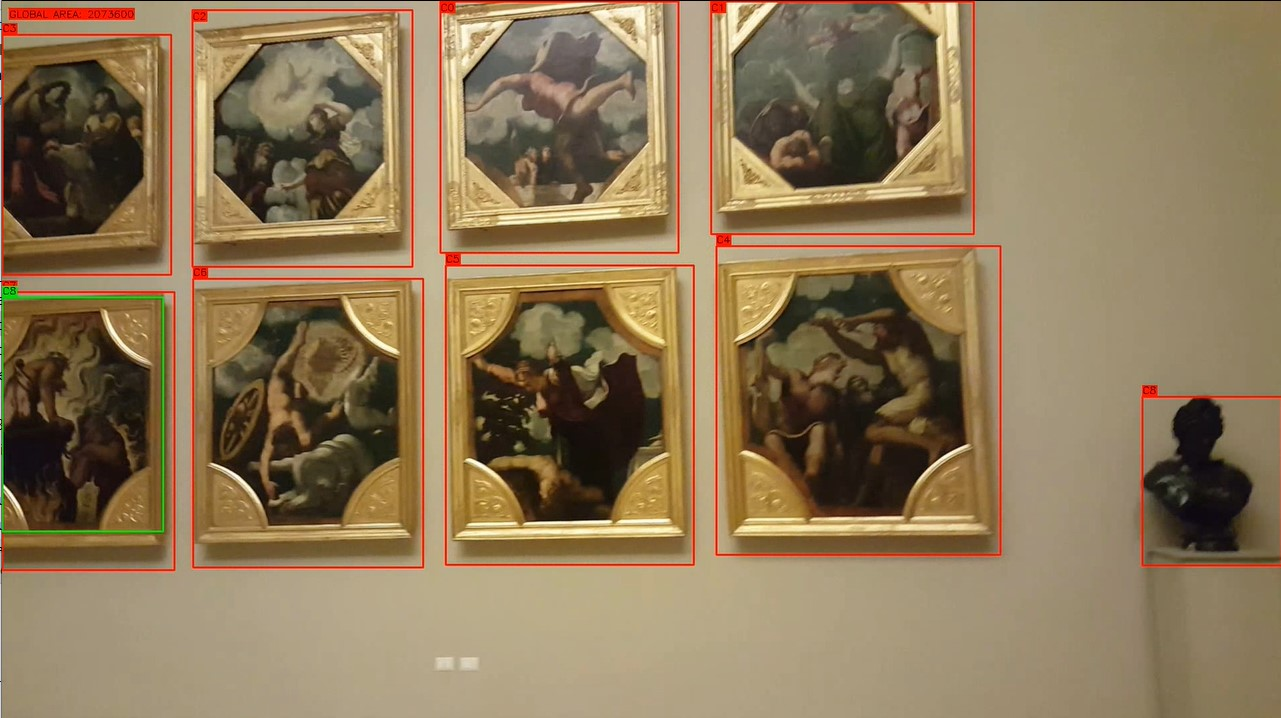
\includegraphics[width=0.6\linewidth]{relevant_rois.jpg}}
    \caption{Relevant ROIs results}
    \label{fig:foobar}
\end{figure}

\subsection{Painting Retrival}
Painting retrival consists in the identification of ROIs passed from the Painting Detection. A ROI is extrapolated from the frame, and it is compared with all the painting in the database:
\begin{itemize}
  \item If the ROI is recognized as one of the painting in the database (with a certain level of security), it's labeled and information to describe it are retrived from the database
  \item If the ROI does not match any painting,  they are classified as ``unidentified object"
\end{itemize}
The comparison is done with ORB \cite{orb}, which is a keypoint detector, just like SIFT and SURF, but not patented.
For every detected ROI, we use ORB to find the keypoint, and we compare them with every keypoints of every painting in the database.
The comparison of the keypoint returns an avarage distance: this distance represent how different are the keypoints found in the considered painting from the keypoints of the ROI; the smaller the distance, the higher the probability that the considered painting from the database is the one that was filmed in the frame.

\subsection{Painting Rectification}
The painting with the smaller average distance from the database, that we will call the ``Best Candidate", may not coincide with the object in the ROI; this may happen for many reasons:
\begin{itemize}
  \item The object is not a painting
  \item The object is a painting, but the quality of that particular frame is very bad (the camera moving, the picture is overexposed to light)
  \item The object is a painting, but is not in the database
\end{itemize}
Painting Rectification can be very helpful: with painting retrival, we select the painting that has the smallest avarage distance from the object in the ROI, then, we try to rectify the object in the frame based on the keypoints of the Best Candidate, and we obtain a rectified image,
if the Best Candidate was actually the painting in the ROI, the rectification should be good, not distored \ref{fig:optimal_rectification}: otherwise, the rectification will bring to a ``Black Hole" \ref{fig:worst_rectification}: a Black Hole happens when the wrong keypoints are used for the rectification.

It can therefore be inferred that a Black Hole happened when our Best Candidate is wrong, it does not concide with the object in the painting.
We can discard the first Best Candidate, and get the painting from the database which has the second smallest average distance.
We repeat the process with the first 10 paintings with smallest average distance, or until we obtain a good rectification.

\begin{figure}
    \centering
    \subfloat[ROI from Painting Detection]{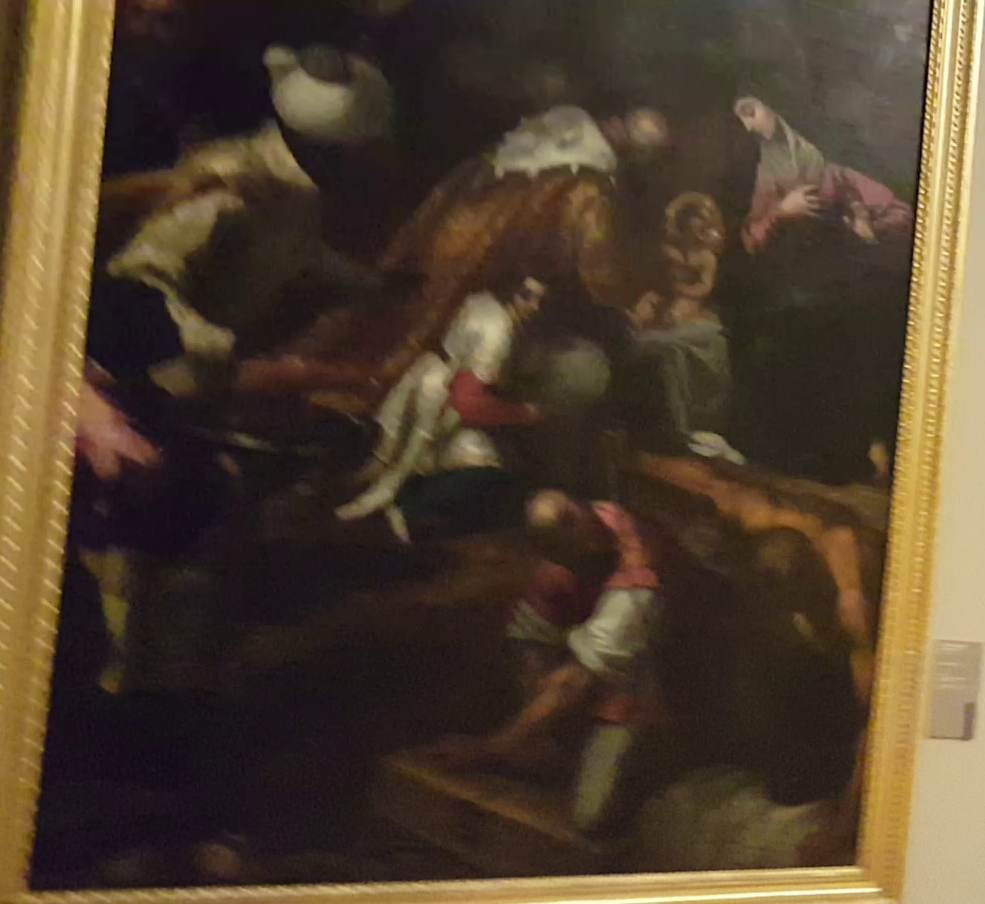
\includegraphics[width=0.33\linewidth]{img_001.png}}
    \subfloat[Keypoints matching]{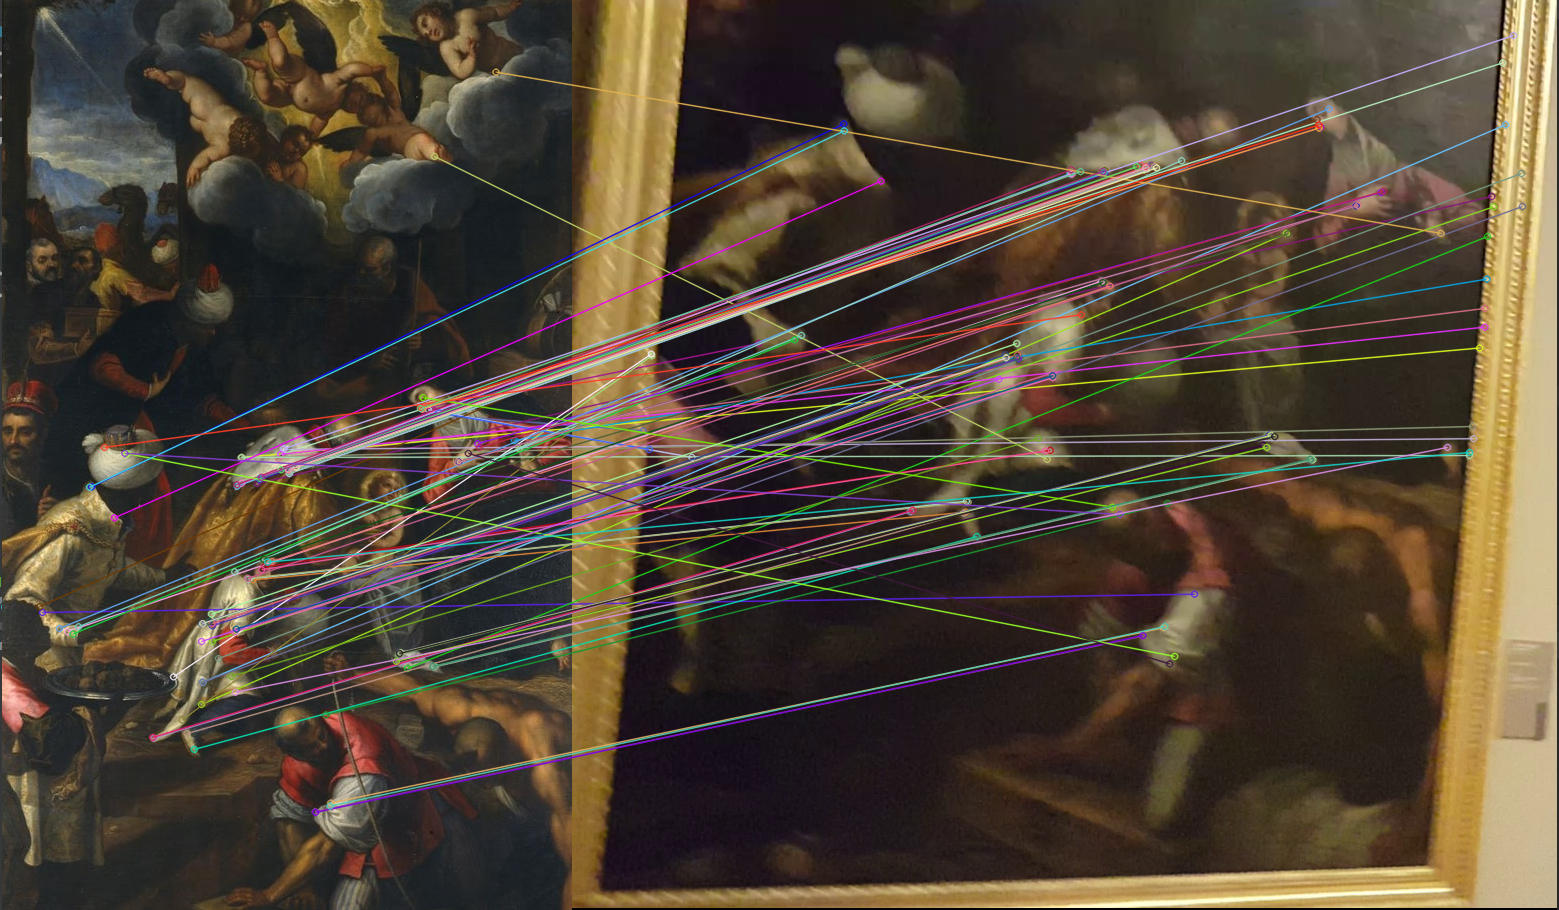
\includegraphics[width=0.33\linewidth]{img_001_KeyPoints.png}}
    \subfloat[Painting rectified from retrived painting]{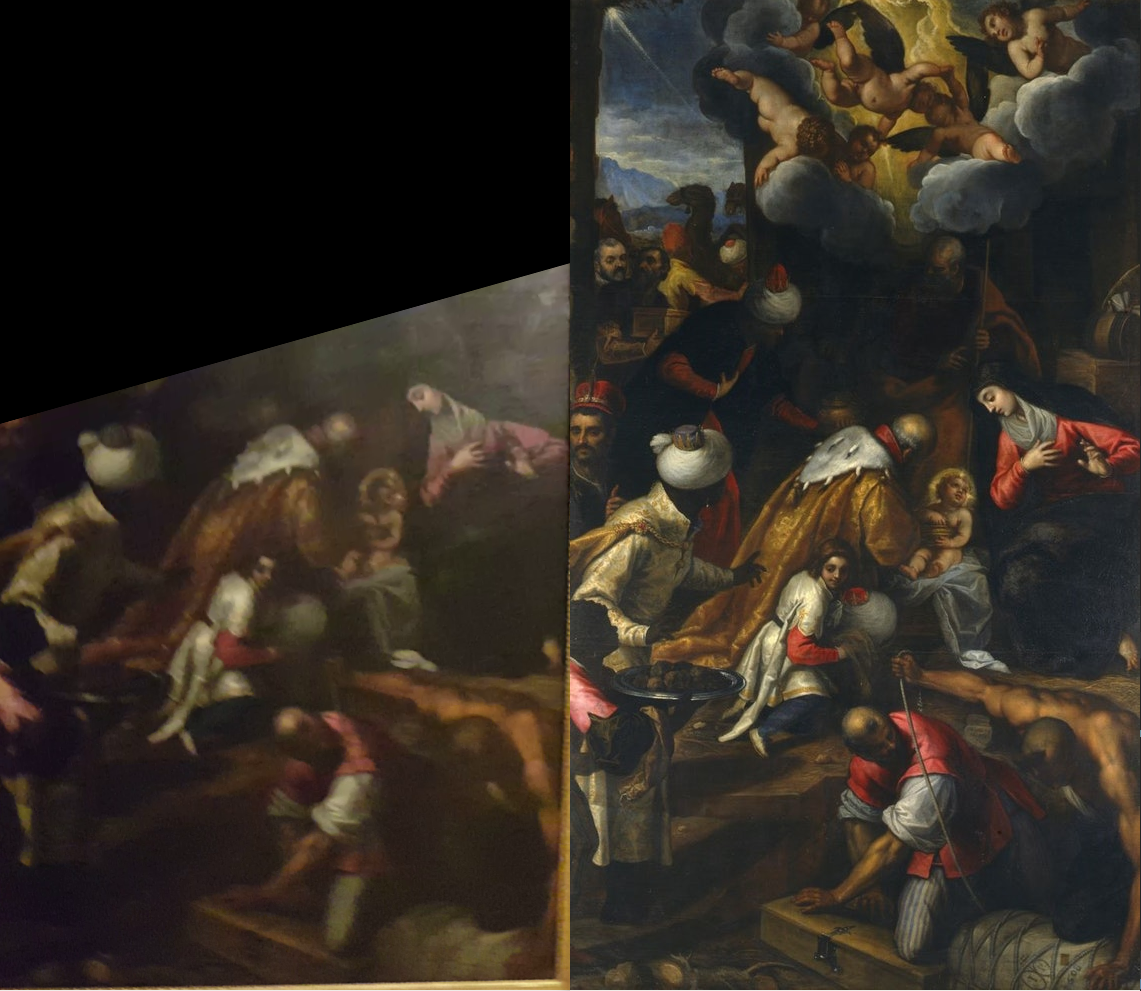
\includegraphics[width=0.33\linewidth]{img_001_RectRetr.png}}
    \caption{Retrival and Rectification optimal case without further corrections}
    \label{fig:optimal_rectification}
\end{figure}

\begin{figure}
    \centering
    \subfloat[Wrong keypoints matching]{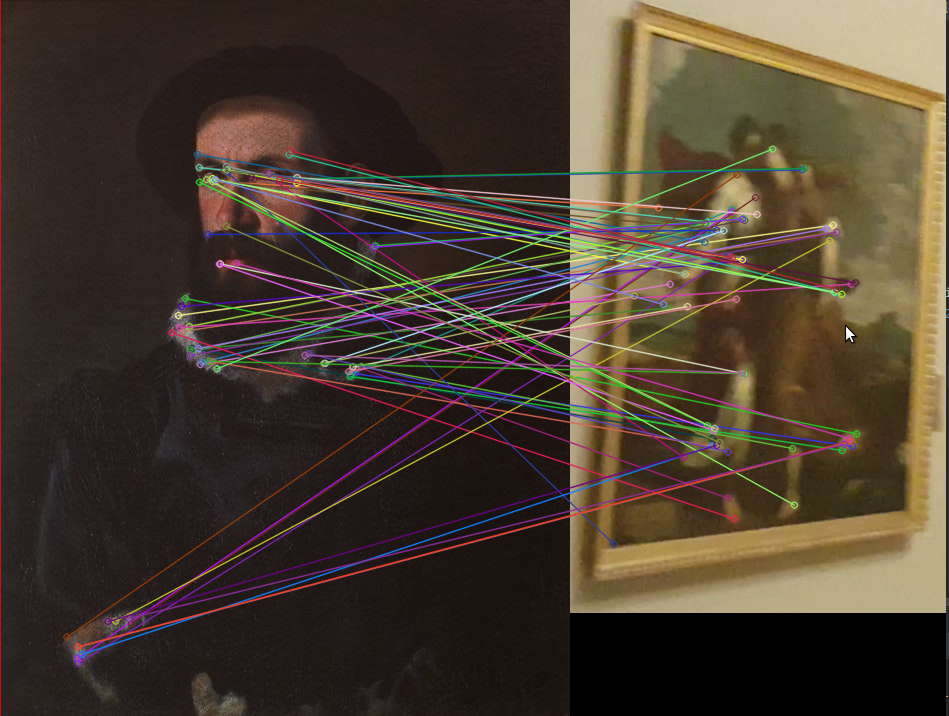
\includegraphics[width=0.5\linewidth]{img_002_wrongdetect.png}}
    \subfloat[Bad rectification: ``Black Hole"]{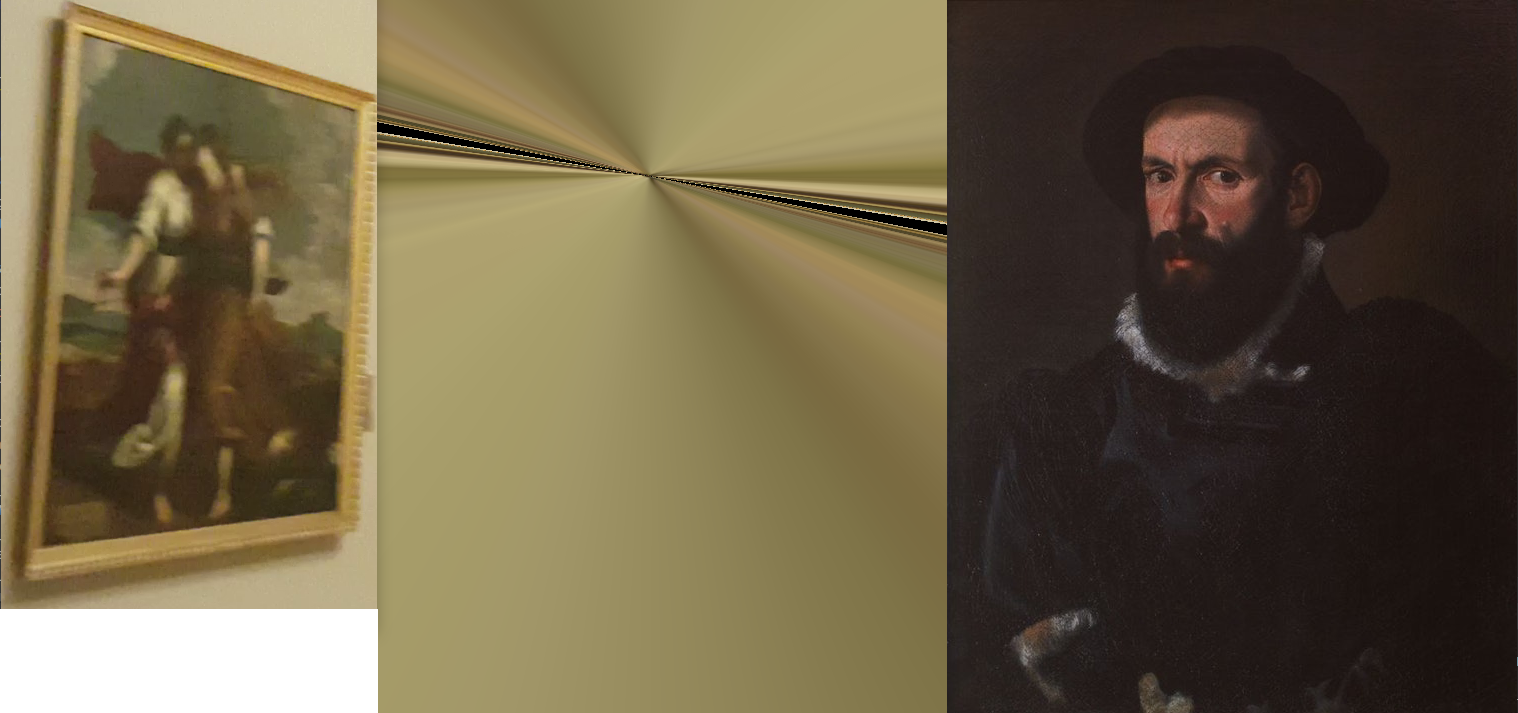
\includegraphics[width=0.5\linewidth]{img_2_Blackhole.png}}\\
    \subfloat[Right keypoints matching]{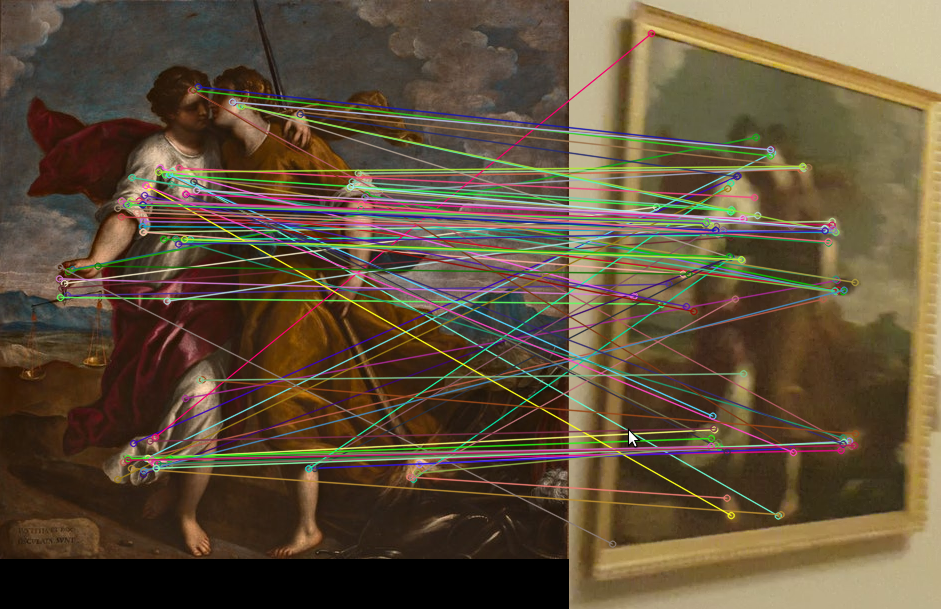
\includegraphics[width=0.5\linewidth]{img_002_right_matches.png}}
    \subfloat[Good rectification]{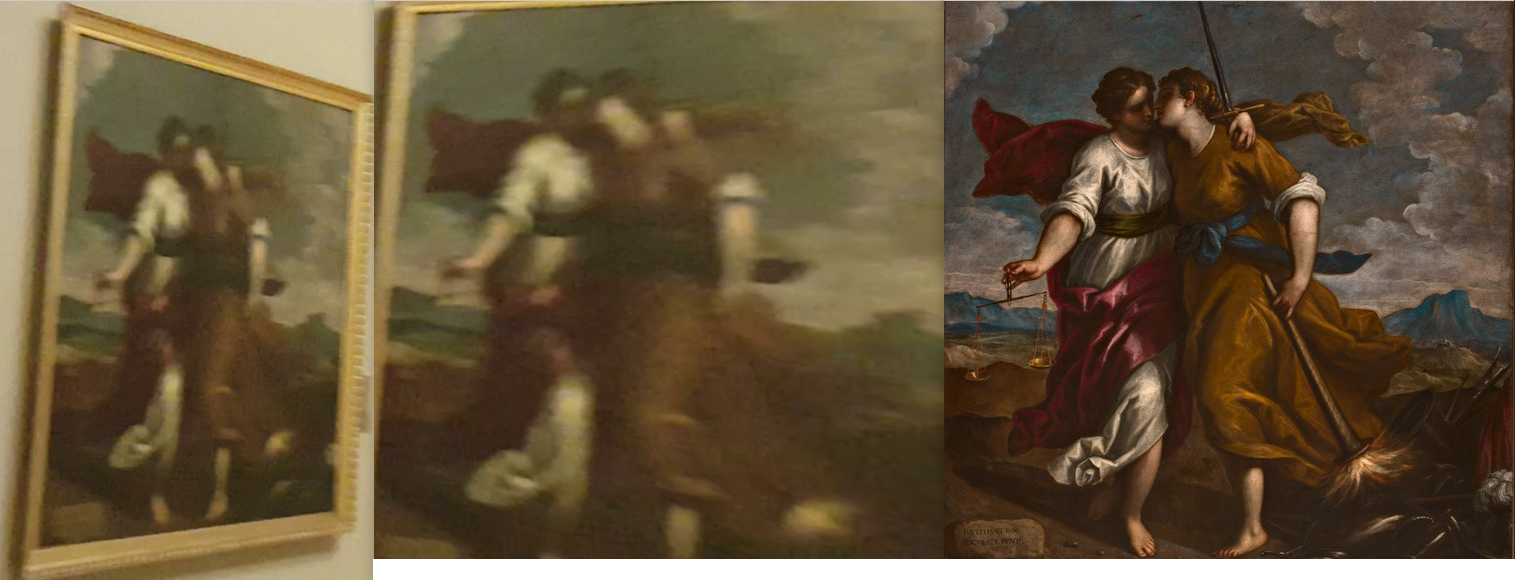
\includegraphics[width=0.5\linewidth]{img_002_goodrect.png}}
    \caption{Retrival and Rectification wrong attempt, correction with keypoint matching and good Rectification}
    \label{fig:worst_rectification}
\end{figure}

Technically, we still use keypoints to detect if the rectified image is a Black Hole. After the rectification, we compute the keypoints on the rectified image: after that, we compute the avarage distance of the keypoints just calculated from the keypoints of the Best Candidate, that we already have. If the rectification was successful, the avarage distance should be low, otherwise it will be high, the rectification was a Black Hole and we have to try with another image.

We set three threshold:
\begin{itemize}
  \item If the average distance is less than 35, it means that we are very confident that we have found the right painting in the database; for this reason, we identify the painting with the information retrieved from the database and we set in which room we are in.
  \item If the average distance is greater than 35, but less than 60, we are pretty sure that we get the right painting, but we are not sure enough to set the room
  \item If the average distance is greater than 60, we are in the situation of a Black Hole, the keypoints are too different, so we have to try with another painting 
\end{itemize}

\subsection{People Detection}

We used YOLOv3 network pre-trained on COCO dataset to detect people on videos, getting the returned
ROIs to draw them on output video.

\subsection{Statue Detection}

To detect the statues in the museum we fine-tuned the YOLOv3 network starting from
weights trained on COCO dataset. At the beginning we thought to detect statues and paintings
to improve the detection made with the Image Processing approach, so we trained the network
on 2 classes: Paintings and Statues.

We made our custom annotated dataset ripping frames from all videos of the museum, storing
them with a step of 250 frames for each video, obtaining 605 images mainly composed by paintings 
with only a 10\% of images containing statues.
We tried to train the network with this small and unbalanced dataset using different {\tt Learning Rate} 
values but the result was unsufficient.

After those tries we thought to use the network only to detect the statues, because the Image Processing
method was still better to detect paintings but often it wasn't able to detect statues.
So we learned the lesson and we tried to balance the dataset selecting manually frames with statues
from videos obtaining 282 images, each containg at least a statue with different point of views.
We annotated those images with more focus on statues than paintings, then we made a simple data 
augmentation script to flip all statues frames, obtaining 564 images with statues.
Finally our dataset contains 1169 images, slightly balanced in number of paintings and statues.

Using Adam optimizer with {\tt Non Maxima Suppression} value of 0.4, {\tt Confidence Threshold} of 0.8 
and a {\tt Learning Rate} of 0.004 we achieved an AP of {\bf 6.39\%}, considering also the painting class that we 
discarded in detection phase. 

To train the network we used an Nvidia GTX 1050 with 4Gb and it took us almost 4 days to
reach the 242th epoch with a batch size of 2, then we just stopped the training due to overfitting on 
{\tt confidence loss} \ref{fig:loss_conf}. 
We achieved the best results of AP with the 177th epoch and we used those weights to detect
statues on videos trying different combinations of {\tt Non Maxima Suppression} and {\tt Confidence Threshold} values,
defining them to 0.1 and 0.98 respectively.

\subsection{Segmentation}
The last section of the project deals with segmentation, both of paintings and Stautes.
We used GrabcCut algorithm as defined in \textit{Carsten Rother, Vladimir Kolmogorov, Andrew Blake} \cite{grabcut}
: exploiting the ROIs received both from Painting Detection and YOLOv3, we were able to use GrabCut algorithm without user interactions.
In particular, we took every ROI extrapolated in each frame, and enlarged them: In this manner, we had a section of the frame, in which we could draw the rectangle to define what was definitely background.
At this point, we used GrabCut to extrapolate what in the ROI was our object of interest, was that a painting or a statue.
We highlighted the objects of interest in green \ref{fig:results2}.

\section{Results}

In this section, some results frame and training graphs will be shown.

\begin{figure}
    \centering
    \subfloat[]{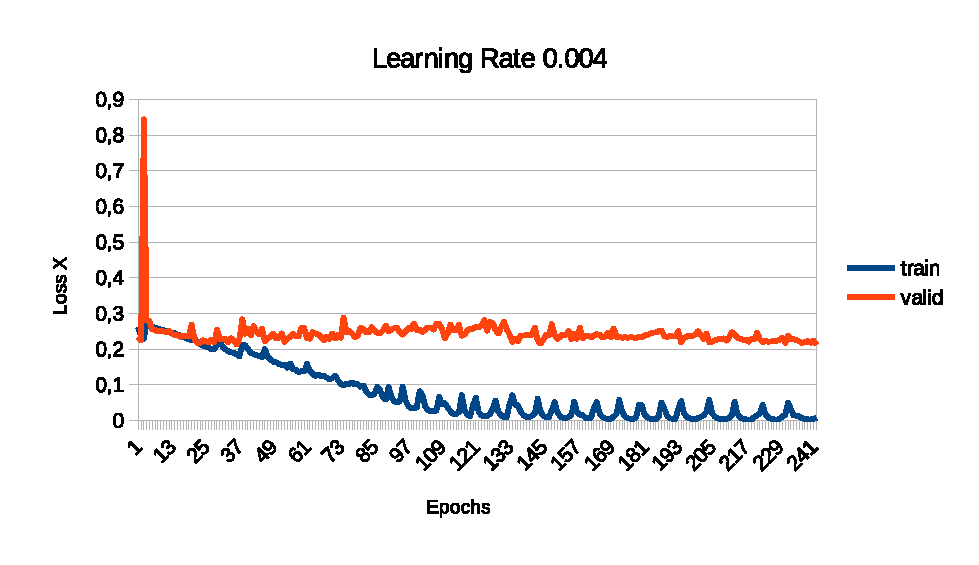
\includegraphics[width=0.5\linewidth]{loss_x.eps}}
    \subfloat[]{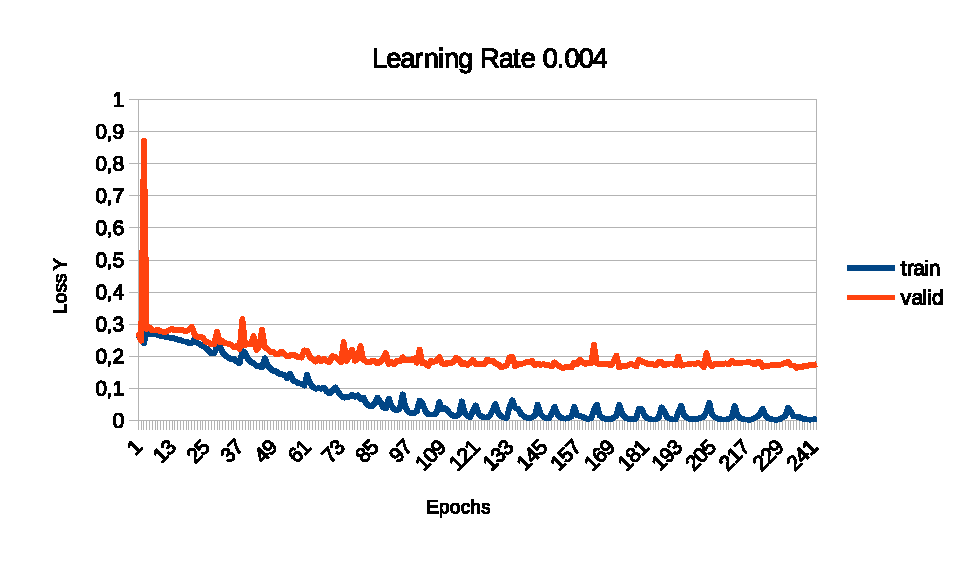
\includegraphics[width=0.5\linewidth]{loss_y.eps}}\\
    \subfloat[]{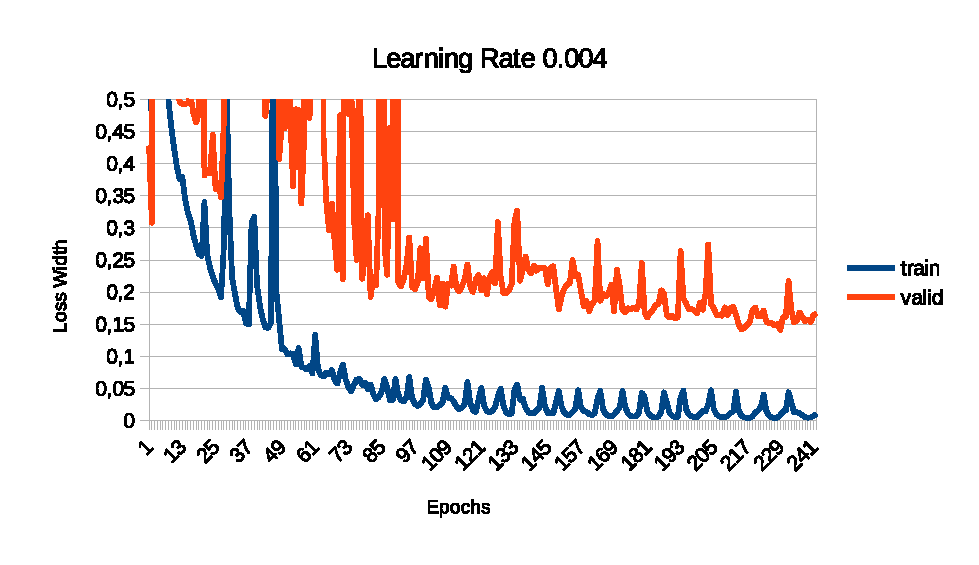
\includegraphics[width=0.5\linewidth]{loss_width.eps}}
    \subfloat[]{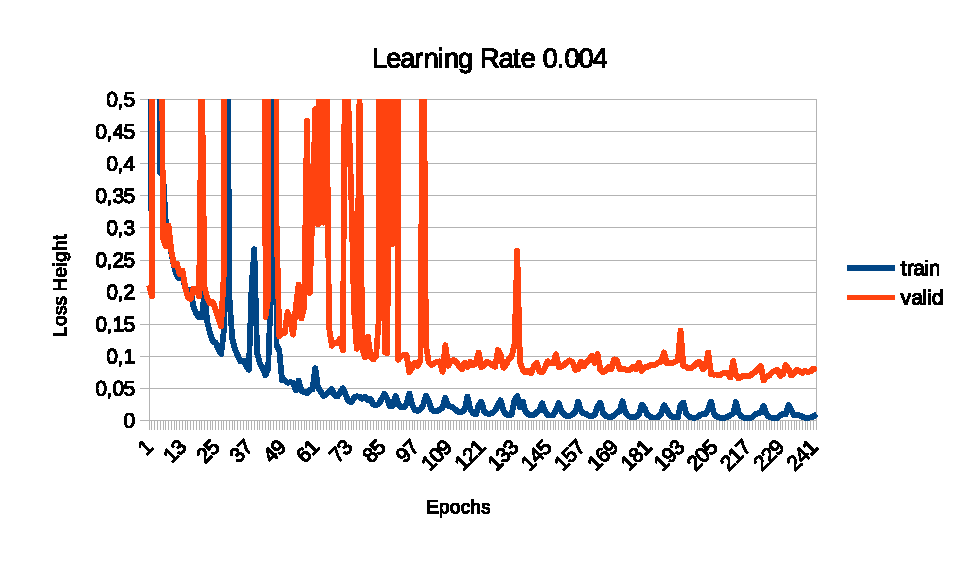
\includegraphics[width=0.5\linewidth]{loss_height.eps}}
    \caption{(a) Loss X, (b) Loss Y, (c) Loss Width and (d) Loss Height}
    \label{fig:localization_loss}
\end{figure}

\begin{figure}[t]
\begin{center}
   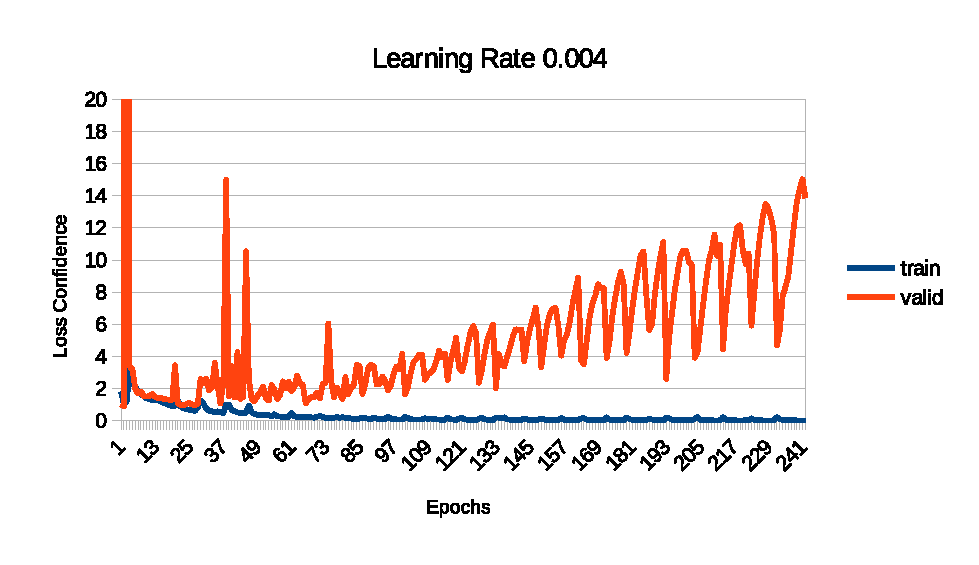
\includegraphics[width=1\linewidth]{loss_conf.eps}
\end{center}
   \caption{The Loss Confidence begins to overfit after few epochs, probably due to bad labeling of
paintings when we expanded the dataset.}
\label{fig:loss_conf}
\label{fig:onecol}
\end{figure}

\begin{figure}[t]
\begin{center}
   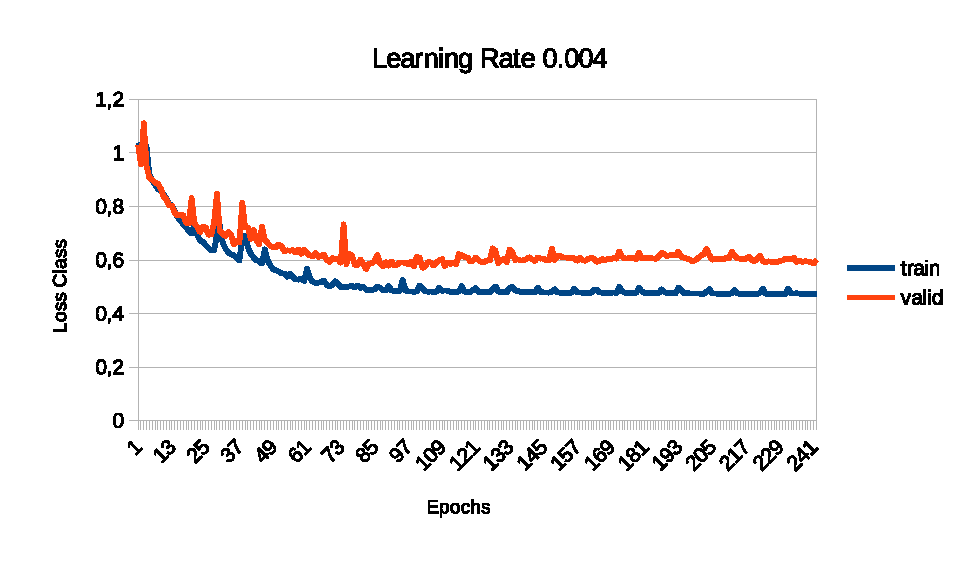
\includegraphics[width=1\linewidth]{loss_class.eps}
\end{center}
   \caption{The Loss Class has a good trend.}
\label{fig:loss_class}
\label{fig:onecol}
\end{figure}

\begin{figure}
    \centering
    \subfloat[]{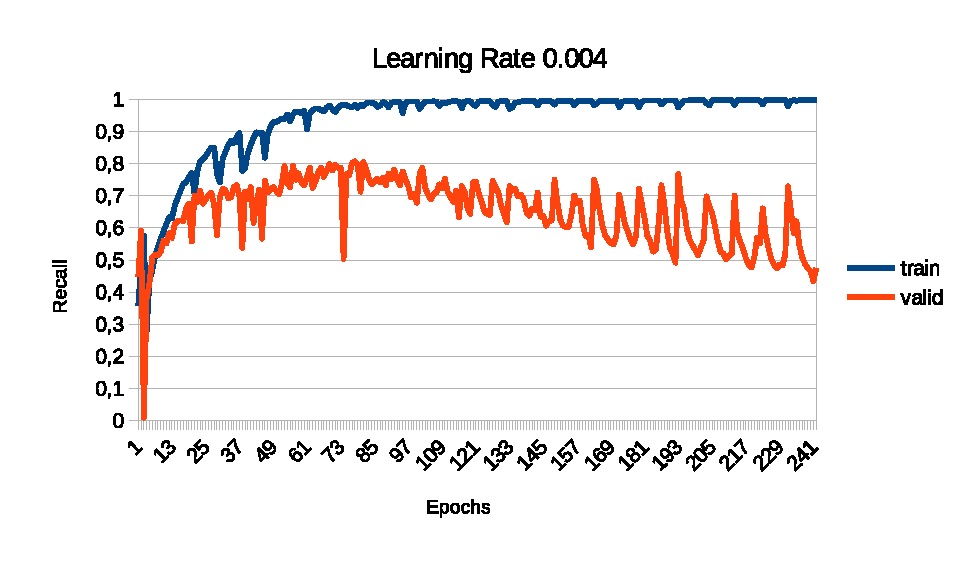
\includegraphics[width=0.5\linewidth]{recall.eps}}
    \subfloat[]{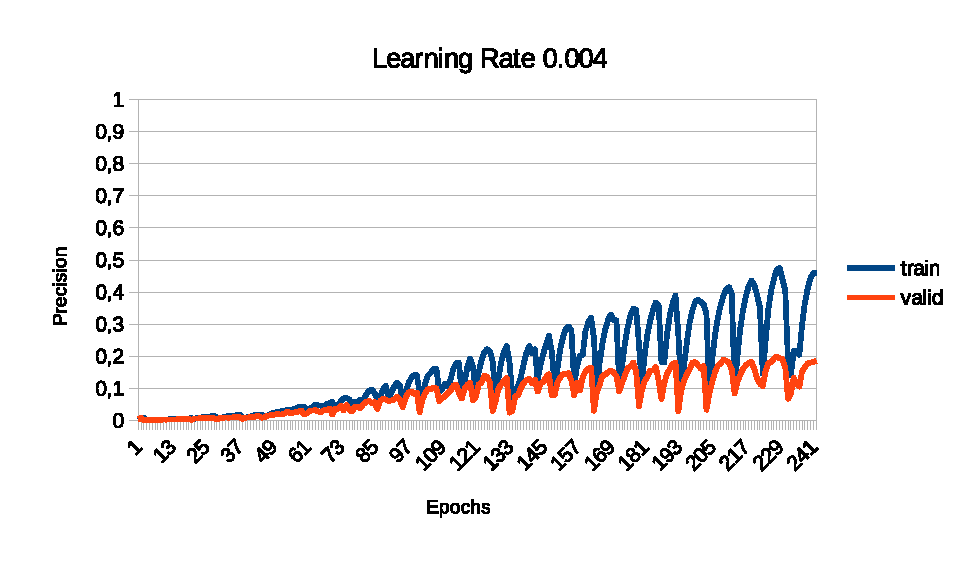
\includegraphics[width=0.5\linewidth]{precision.eps}}
    \caption{(a) Recall  and (b) Precision curves}
    \label{fig:recall_precision}
\end{figure}

\begin{figure}[t]
\begin{center}
   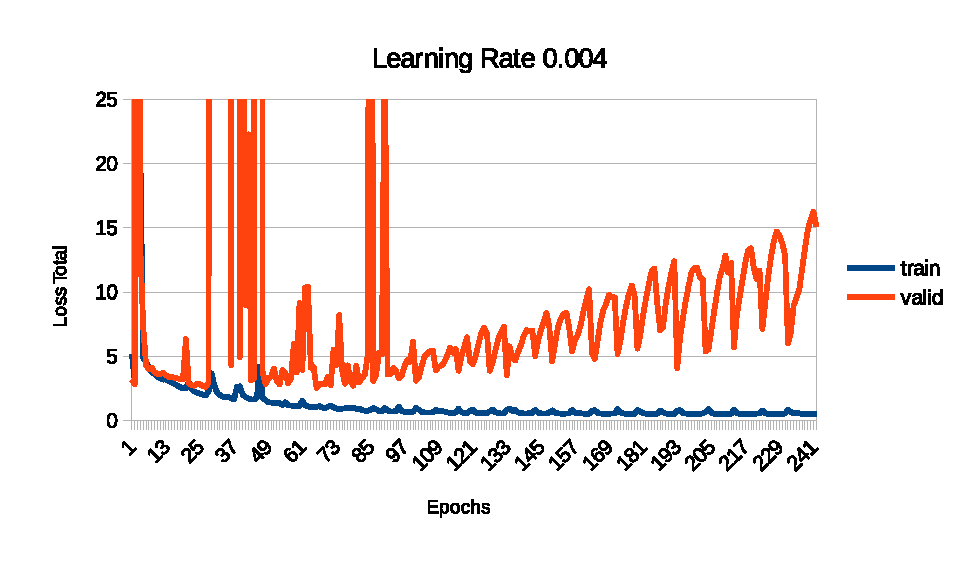
\includegraphics[width=1\linewidth]{loss_total.eps}
\end{center}
   \caption{The Total Loss is affected mainly by the loss confidence curve \ref{fig:loss_conf}, 
while the loss class \ref{fig:loss_class} and localization losses \ref{fig:localization_loss} are good enough to improve the precision \ref{fig:recall_precision}.}
\label{fig:loss_total}
\label{fig:onecol}
\end{figure}

\begin{figure*}[t]
\begin{center}
    \subfloat[No otsu\_optimization, bad]{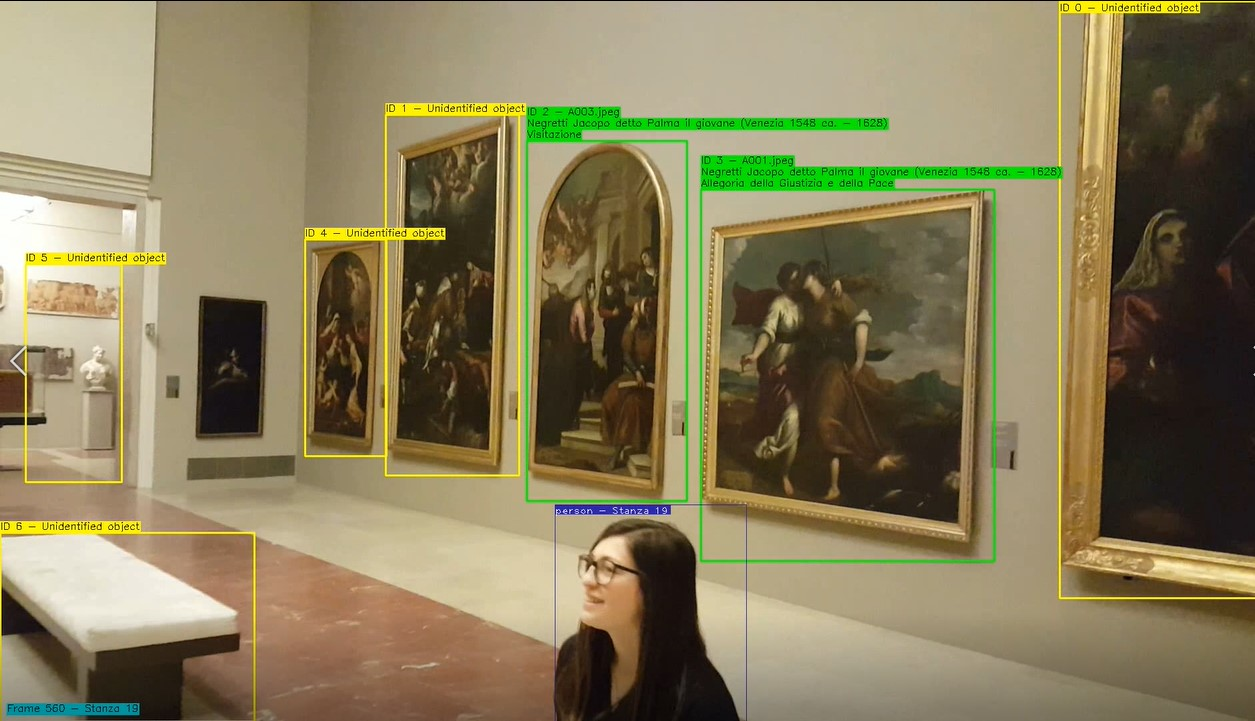
\includegraphics[width=0.5\linewidth]{4720_Frame560_noOtsu_bad.jpg}}
    \subfloat[With otsu\_optimization, good]{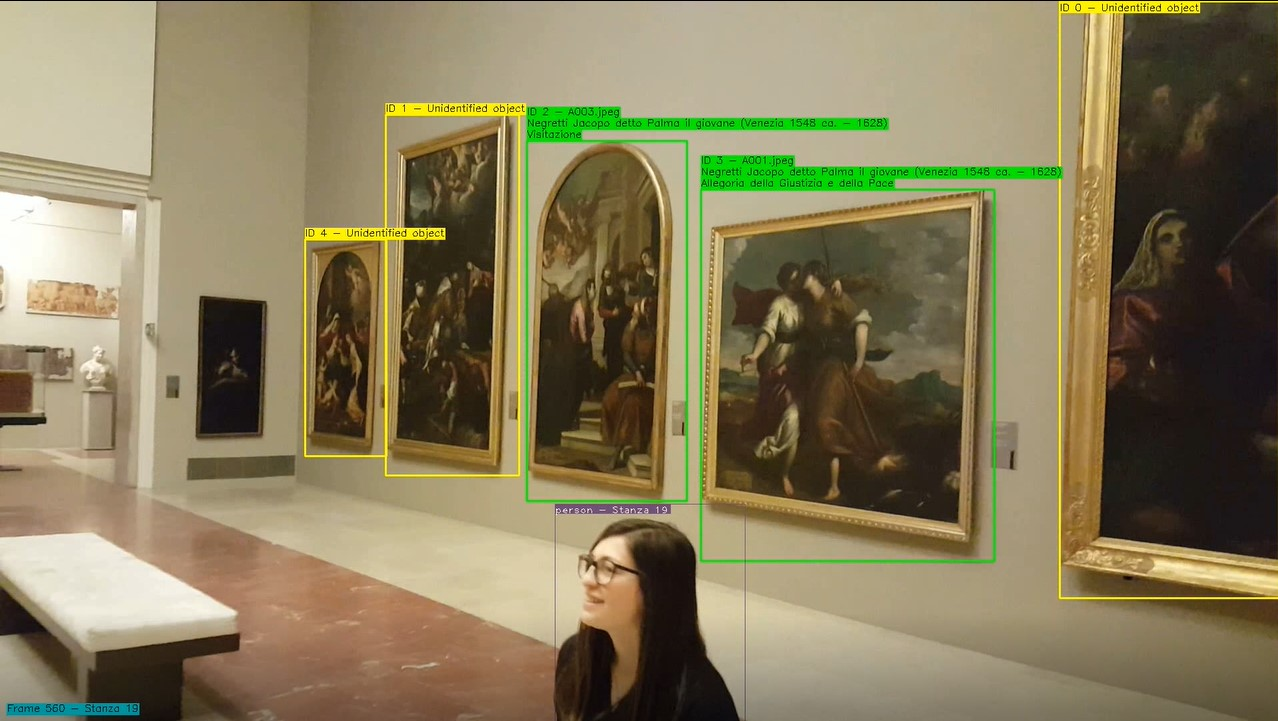
\includegraphics[width=0.5\linewidth]{4720_Frame560_yesOtsu_good.jpg}}\\
    \subfloat[No otsu\_optimization, good]{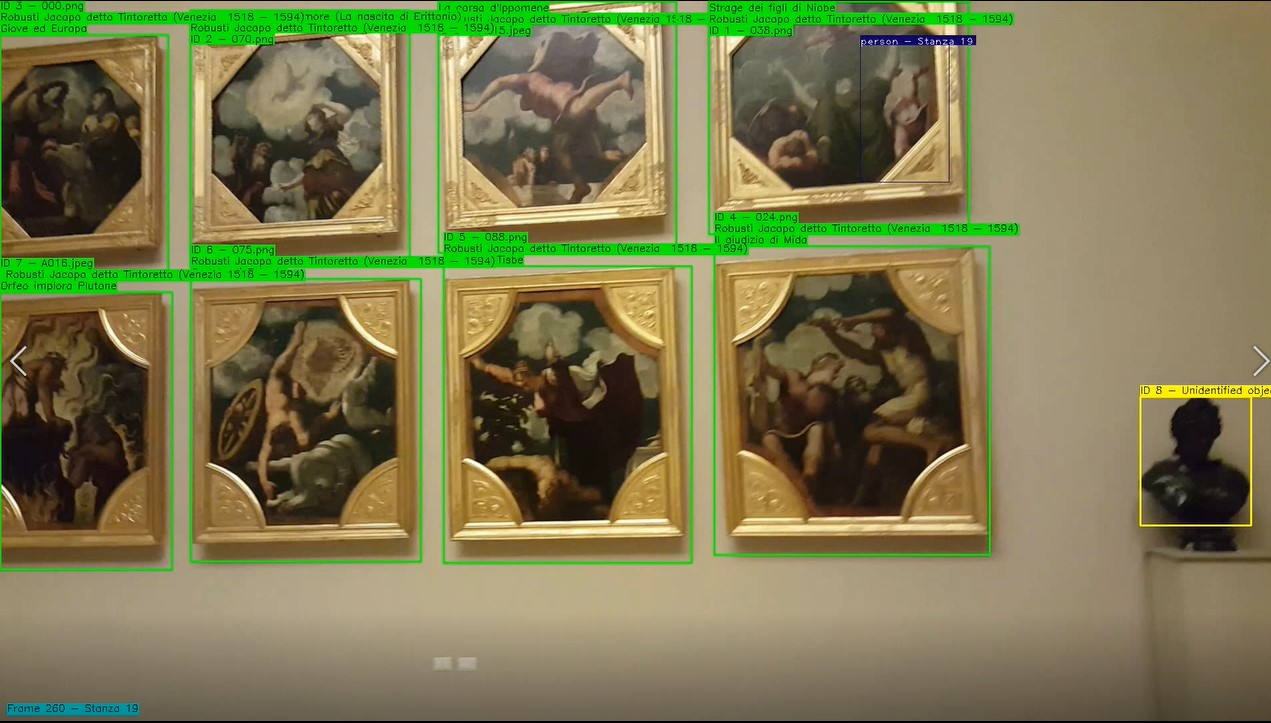
\includegraphics[width=0.5\linewidth]{4720_Frame260_noOtsu_Good.jpg}}
    \subfloat[With otsu\_optimization, bad]{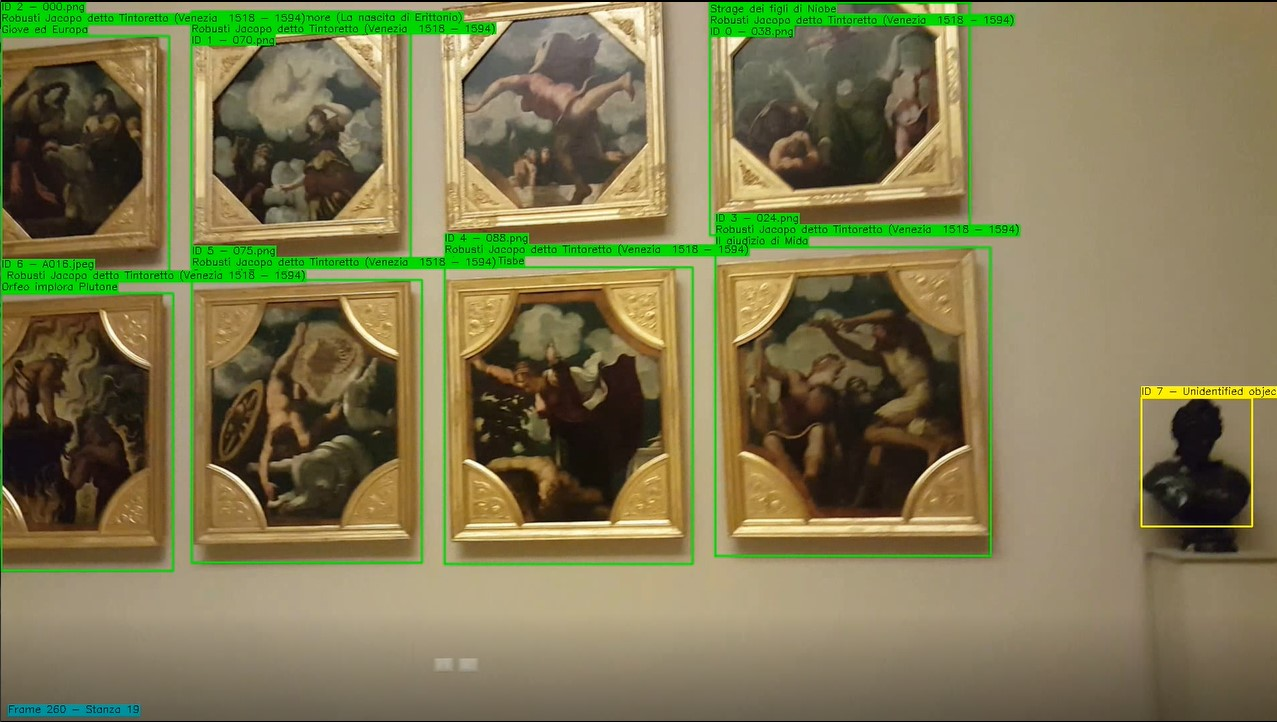
\includegraphics[width=0.5\linewidth]{4720_Frame260_yesOtsu_bad.jpg}}
\end{center}
   \caption{Example of otsu\_optimization (no statue detection nor segmentation)}
\label{fig:results1}
\end{figure*}

\begin{figure*}
    \centering
    \subfloat[]{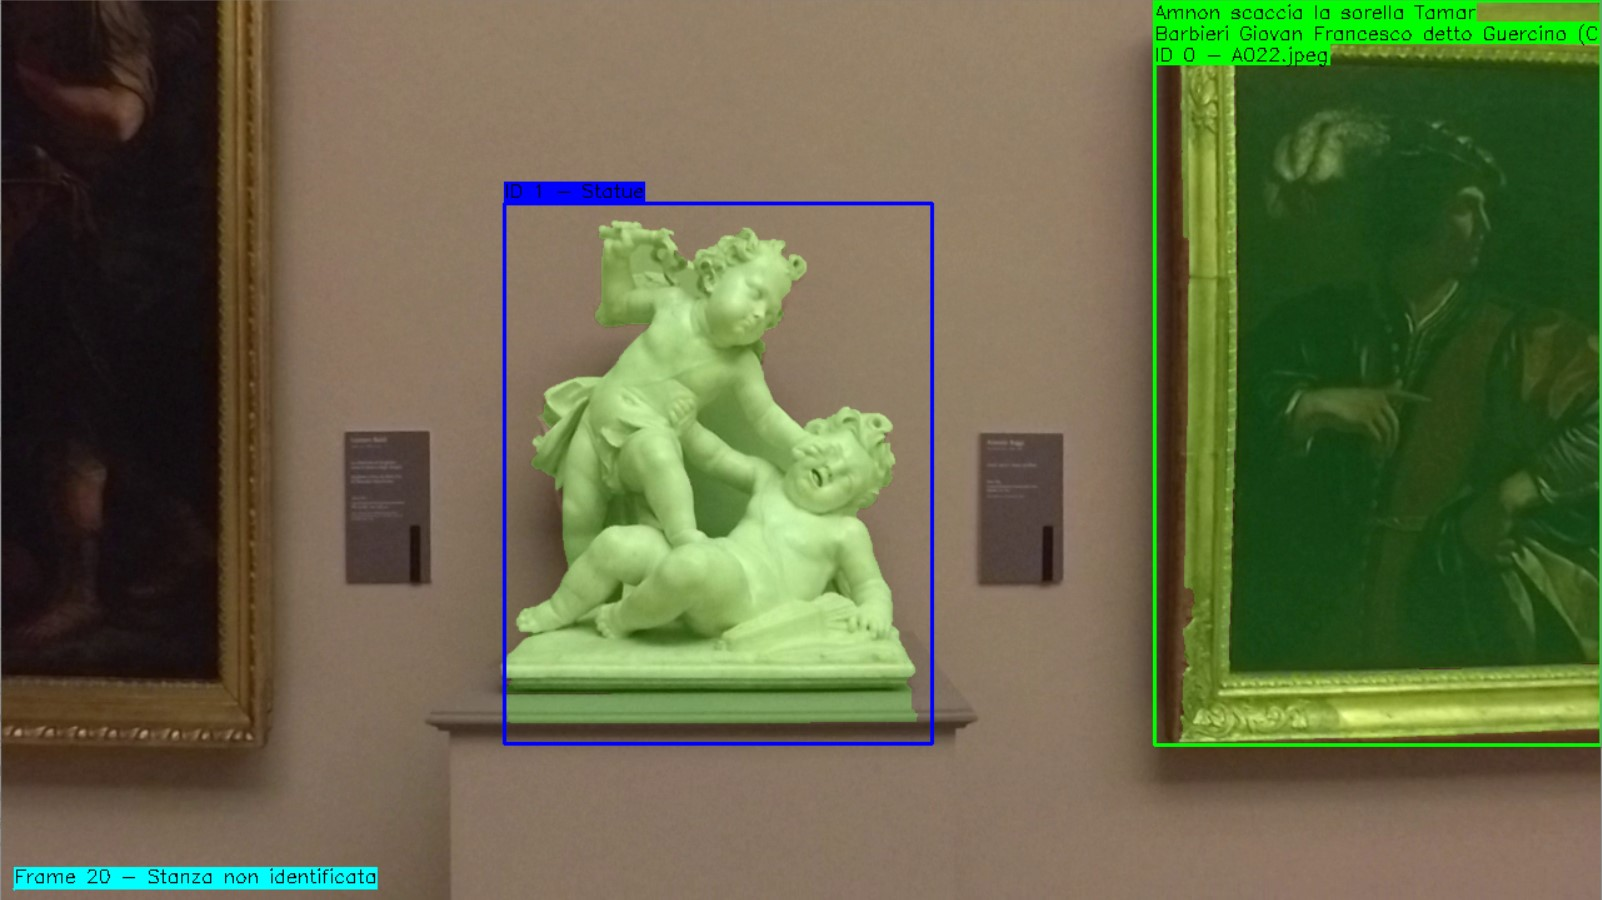
\includegraphics[width=0.5\linewidth]{good_segm_det_frame_20.jpg}}
    \subfloat[]{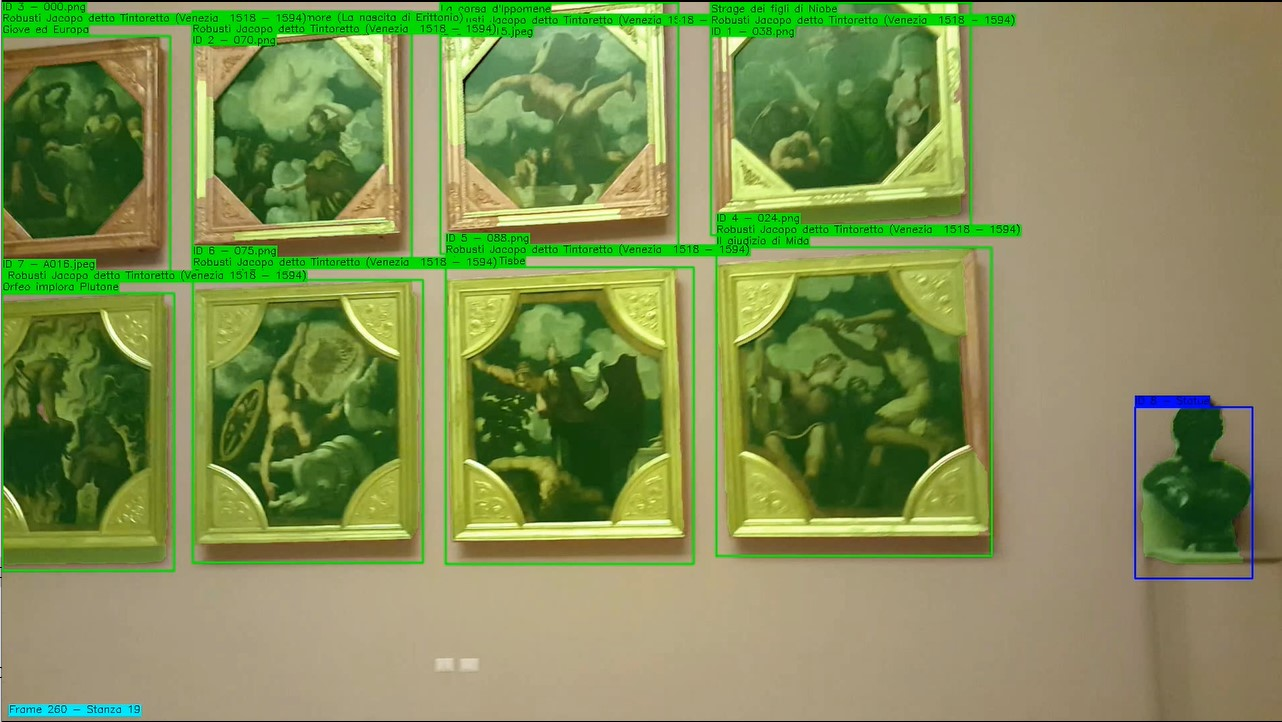
\includegraphics[width=0.5\linewidth]{good_segmentation2.jpg}}
    \caption{Example of segmentation and statue detection}
    \label{fig:results2}
\end{figure*}

\section{Discussion}

Considering this is our first work on this kind of problems we know that we could achieve better results with more work and time.
In particular we could improve our network detection with a wider and more balanced dataset.
Furthermore we could improve our painting detection discarding some useless ROIs (\eg the labels describing paintings and statues) using some Image Processing technique (\eg Histogram to discard labels).
We know also that Retrival, Rectification and Detection tasks could work better if we had a complete paintings and statues database.

{\small
\bibliographystyle{ieee_fullname}
\bibliography{egbib}
}

\end{document}
